\documentclass[UTF8]{beamer}
\mode<presentation> {
	\usetheme{Boadilla}
}
\setbeamertemplate{navigation symbols}{}
\usepackage[utf8]{inputenc}
\usepackage[spanish]{babel}
\usepackage{graphicx}
\graphicspath{{images/}}


\title[Portada]{
	Galera Cluster \\
	\large "Un verdadero multi-master sin que se rompa a los 3 minutos"\\
}
\author{Chema Alcaraz}
\date{2 de Febrero de 2017}
\titlegraphic{
\includegraphics[width=4cm]{devops_murcia}}




\begin{document}
	
\begin{frame}
	\titlepage
\end{frame}

\title{¿Quien soy?}

\begin{frame}
	\centering
	\mbox{¿Quien soy?}	
\end{frame}


\begin{frame}
\begin{columns}
    \begin{column}{0.6\textwidth}
        \begin{itemize}
            \item \textbf{Jose Maria Alcaraz (Chema Alcaraz)}
            \item Admin. Sistemas en Ortopedia Plus
            \item Medalla de Plata en SpainSkills 2013
			\item Ganador accésit Redes V Olimpiada Regional 2012
			\item Certificado por Apple como \\'Apple Product Professional' 2011
            \item Ganador IV Olimpiada FP Regional 2010
        \end{itemize}
    \end{column}
    \begin{column}{0.40\textwidth}
        
\includegraphics[width=5cm]{images/yo}
    \end{column}
\end{columns}
	
\end{frame}


\title{¿Que es Galera Cluster?}

\begin{frame}
	\centering
	\mbox{¿Que es?}	
\end{frame}


\begin{frame}
	\frametitle{¿Que es galera?}
\end{frame}

\title{¿Que ganamos con Galera?}
\begin{frame}
	\frametitle{¿Que ganamos con Galera?}
	\begin{itemize}
		\item Replicación sincrona
		\pause
		\item Topología multi-master real
		\pause
		\item Control automático de miembros del cluster
		\pause
		\item Fácil unión de nuevos miembros
		\pause
		\item Replicación paralela a nivel de fila
	\end{itemize}
\end{frame}



\title[Limitaciones]{Limitaciones}
\begin{frame}
	\frametitle[Limitaciones]{Limitaciones}
	\begin{itemize}
		\item La replicación solo funciona con InnoDB
		\pause
		\item Los bloqueos explícitos no están soportados
		\pause
		\item Todas las tablas deben llevar PRIMARY KEY
		\pause
		\item Query log debe ir a un fichero.
		\pause
		\item Las transacciones XA no están soportadas
		\pause
		\item Tamaño de la transacción.
	\end{itemize}
\end{frame}


\title[Backup]{Backup}

\begin{frame}
	\centering
	\mbox{¿Y que pasa con los backups?}	
\end{frame}

\begin{frame}
	\centering
	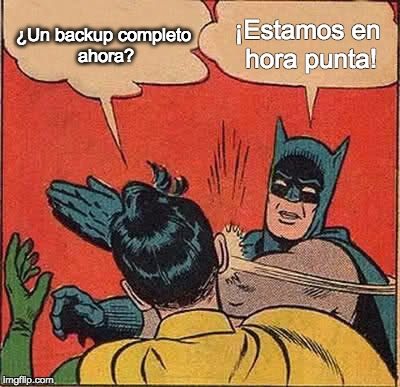
\includegraphics[width=\textwidth,height=\textheight,keepaspectratio]{necesitas_backup}
\end{frame}

\begin{frame}
	
\includegraphics[width=\textwidth,height=\textheight,keepaspectratio]{bloquear}
\end{frame}

\begin{frame}
	
\includegraphics[width=\textwidth,height=\textheight,keepaspectratio]{tenemos_xtrabackup}	
	
\end{frame}
	
	
	
	
	
	
\end{document}